\section{Signals and slots}

\begin{frame}
  \frametitle{The Signals and Slots mechanism}
  \small
  \begin{itemize}
    \item Alternative to events
    \item Common problem in GUI applications:
    \begin{itemize}
      \item How to connect a user action in the GUI, or any other logical event
      in the running application to a piece of code handling the event?
      \begin{figure}[!t]
      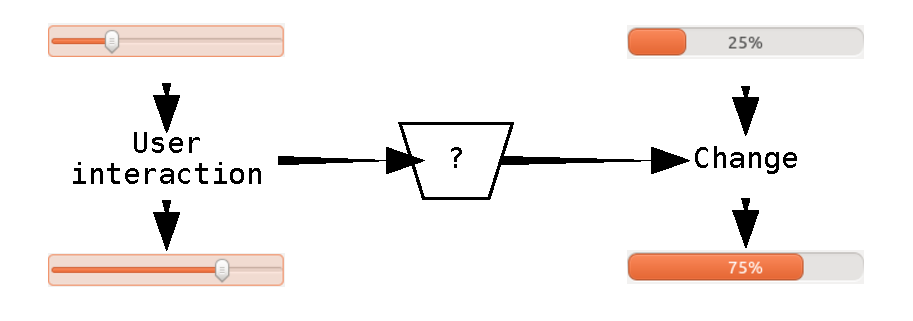
\includegraphics[width=0.8\textwidth]{images/sig_slot_diag1.pdf}
      \end{figure}
    \end{itemize}
    \item Several possible solutions
    \begin{itemize}
      \item Callbacks
      \item The Observer pattern
      \item \ldots
    \end{itemize}
  \end{itemize}
\end{frame}

\begin{frame}
  \frametitle{The Signals and Slots mechanism}
  \small
  \begin{itemize}
    \item Qt's solution to the original problem:
    \begin{itemize}
      \item Implemented by \texttt{QObject} with the help of \texttt{moc}.
      \item Changes in objects {\em emit} various function-like {\em signals}.
      \item Objects can implement special functions -- {\em slots}.
      \item Connections can be created between signals and slots.
      \begin{itemize}
        \footnotesize
        \item The signatures of signal and slot must match.
        \item One signal can be connected to many slots.
        \item Many signals can be connected to a single slot.
        \item When a signal is emitted the connected slots -- functions are called.
      \end{itemize}
    \end{itemize}
  \end{itemize}
  \begin{figure}[!t]
  \centering
  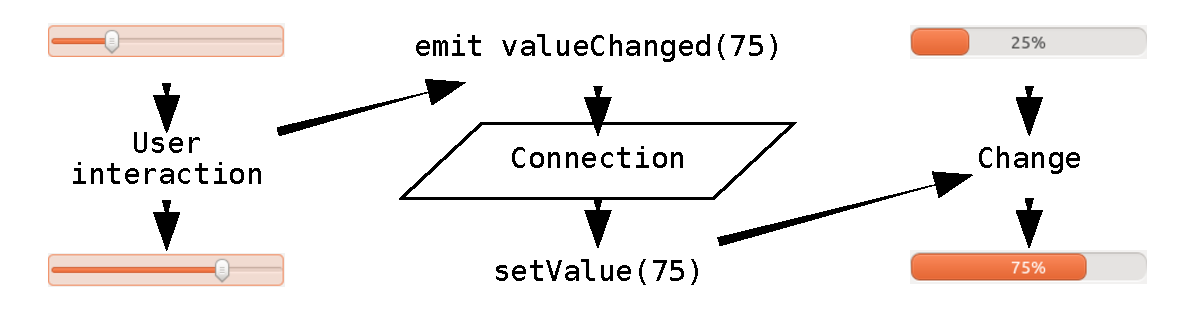
\includegraphics[width=\textwidth]{images/sig_slot_diag2.pdf}
  \end{figure}
\end{frame}

\begin{frame}[fragile]
  \frametitle{Declaring and implementing signals and slots}
  \footnotesize
  \begin{itemize}
    \item Header file
    \begin{itemize}
      \item Class declaration -- must inherit from \texttt{QObject}:
        \begin{lstlisting}[basicstyle=\scriptsize\ttfamily]
	class MyClass : public QObject {
	    Q_OBJECT // triggers the moc
	(*@\alert{signals}@*): // signal declarations
	    void stringChanged(const QString&);
	(*@\alert{public slots}@*): // slot declarations
	    void updateString(const QString&); 
	};\end{lstlisting}
    \end{itemize}
    \item Source file
    \begin{itemize}
      \item The signal code is implemented by \texttt{moc}.
      \item Signal emission:
      \begin{lstlisting}[basicstyle=\scriptsize\ttfamily]
	(*@\alert{emit}@*) stringChanged(string);
	\end{lstlisting}
      \item Manual slot implementation:
      \begin{lstlisting}[basicstyle=\scriptsize\ttfamily]
	void MyClass::updateString(const QString& str) {
	    // handle the action
	}\end{lstlisting}
    \end{itemize}
  \end{itemize}
\end{frame}

\begin{frame}[fragile]
  \frametitle{Connecting and disconnecting signals and slots}
   \begin{itemize}
     \item Connecting
     \begin{itemize}
      \item The \verb@QObject::connect@ overloaded member functions.
      \item General purpose: connects a particular signal of \verb@sender@ to a
        particular slot of \verb@receiver@, optionally specifying the connection
        \verb@type@.
      \item All overloads of \verb@connect@ return an instance of
        \verb@QMetaObject::Connection@\footnote
         {\url{http://doc.qt.io/qt-5.6/qmetaobject-connection.html}}:
      \begin{itemize}
        \item Representation of a signal-slot connection.
        \item It can be used to disconnect the connection, or check if
          the connection is valid.
      \end{itemize}
      \item If the sender or receiver are destroyed, the connection is automatically
        disconnected.
     \end{itemize}
     \item Disconnecting
     \begin{itemize}
       \item The \verb@QObject::disconnect@ overloaded member functions.
     \end{itemize}
    \end{itemize}
\end{frame}

\begin{frame}[fragile]
  \frametitle{Connection types -- \texttt{ConnectionType}\footnote
    {\url{http://doc.qt.io/qt-5.6/qt.html\#ConnectionType-enum}}}
  \begin{center}
  \tiny
  \rowcolors{2}{green!80!yellow!50}{green!70!yellow!40}
  \begin{tabular}{|p{0.30\textwidth}|p{0.60\textwidth}|}
    \hline
    \textbf{Class} & \textbf{Description} \\
    \hline
    \texttt{Qt::AutoConnection} & If the receiver lives in the thread that emits
      the signal, \texttt{Qt::DirectConnection} is used.
      Otherwise, \texttt{Qt::QueuedConnection} is used. The actual connection
      type is determined when the signal is emitted. \\
    \hline
    \texttt{Qt::DirectConnection} & The slot is invoked immediately when the signal
      is emitted. The slot is executed in the signaling thread. \\
    \hline
    \texttt{Qt::QueuedConnection} & The slot is invoked when control returns to
      the event loop of the receiver's thread. The slot is executed in the
      receiver's thread. \\
    \hline
    \texttt{Qt::BlockingQueuedConnection} & Same as \texttt{Qt::QueuedConnection},
      except that the signaling thread blocks until the slot returns. This
      connection must not be used if the receiver lives in the signaling thread,
      or else the application will deadlock. \\
    \hline
    \texttt{Qt::UniqueConnection} & This is a flag that can be combined with any
      one of the above connection types, using the bitwise OR operator.
      When \texttt{Qt::UniqueConnection} is set, \verb@QObject::connect@ will fail
      if the connection already exists (if the same signal is already connected
      to the same slot for the same pair of objects). \\
    \hline
  \end{tabular}
  \end{center}
\end{frame}

\begin{frame}[fragile]
  \frametitle{Connecting signals and slots (cont.)}
   \begin{itemize}
      \item Purpose: connects a named signal of \verb@sender@ to a named slot
        of \verb@receiver@, optionally specifying the connection \verb@type@.
      \item Declaration
      \begin{lstlisting}[basicstyle=\scriptsize\ttfamily]
	QMetaObject::Connection QObject::connect(
	    const QObject *sender, const char *signal_name,
	    const QObject *receiver, const char *slot_name,
	    Qt::ConnectionType type = Qt::AutoConnection
	);
      \end{lstlisting}
      \item Usage
      \begin{lstlisting}[basicstyle=\scriptsize\ttfamily]
	QObject* sender = ...;
	QObject* receiver = ...;
	QObject::connect(
	    sender, SIGNAL(signalFunc(Type1, Type2, ...)),
	    receiver, SLOT(handleFunc(Type1, Type2, ...)),
	    Qt::AutoConnection
	);
      \end{lstlisting}
    \end{itemize}
\end{frame}

\begin{frame}[fragile]
  \frametitle{Connecting signals and slots (cont.)}
   \begin{itemize}
      \item Purpose: connects a named signal of \verb@sender@ to a named slot
        of \verb@this@ instance, optionally specifying the connection \verb@type@.
      \item Declaration
      \begin{lstlisting}[basicstyle=\scriptsize\ttfamily]
	QMetaObject::Connection QObject::connect(
	    const QObject *sender, const char *signal_name,
	    const char *slot_name,
	    Qt::ConnectionType type = Qt::AutoConnection
	);
      \end{lstlisting}
      \item Usage
      \begin{lstlisting}[basicstyle=\scriptsize\ttfamily]
	QObject* receiver = ...;
	this->connect(
	    sender, SIGNAL(signalFunc(Type1, Type2, ...)),
	    SLOT(handleFunc(Type1, Type2, ...))
	);
      \end{lstlisting}
    \end{itemize}
\end{frame}

\begin{frame}[fragile]
  \frametitle{Connecting signals and slots (cont.)}
   \begin{itemize}
      \item Purpose: connects a named signal of \verb@sender@ to the specified
        \verb@functor@.
      \item Declaration
      \begin{lstlisting}[basicstyle=\scriptsize\ttfamily]
	QMetaObject::Connection QObject::connect(
	    const QObject *sender,
	    PointerToMemberFunction signal,
	    Functor functor
	);
      \end{lstlisting}
      \item Usage
      \begin{lstlisting}[basicstyle=\scriptsize\ttfamily]
	void clickHandler(void);
	QPushButton *sender = new QPushButton;
	QObject::connect(
	    sender, &QPushButton::clicked,
	    clickHandler
	);
      \end{lstlisting}
    \end{itemize}
\end{frame}

\begin{frame}[fragile]
  \frametitle{Connecting signals and slots (cont.)}
   \begin{itemize}
      \item Purpose: connects a signal member function of \verb@sender@ to
        a slot member function of \verb@receiver@, optionally specifying the
        connection type.
      \item Declaration
      \begin{lstlisting}[basicstyle=\scriptsize\ttfamily]
	QMetaObject::Connection QObject::connect(
	    const QObject *sender,
	    PointerToMemberFunction signal,
	    const QObject *receiver,
	    PointerToMemberFunction handler,
	    Qt::ConnectionType type = Qt::AutoConnection
	);
      \end{lstlisting}
      \item Usage
      \begin{lstlisting}[basicstyle=\scriptsize\ttfamily]
	QLabel *sender = new QLabel();
	QLineEdit *receiver = new QLineEdit();
	QObject::connect(
	    lineEdit, &QLineEdit::textChanged,
	    label,    &QLabel::setText
	);
      \end{lstlisting}
    \end{itemize}
\end{frame}

\begin{frame}[fragile]
  \frametitle{Connecting signals and slots (cont.)}
   \begin{itemize}
      \item Purpose: connects a signal member function of \verb@sender@ the
        specified \verb@functor@. The connection is handled in the event loop
        of a specific \verb@context@ object -- typically a parent widget.
      \item Declaration
      \begin{lstlisting}[basicstyle=\scriptsize\ttfamily]
	QMetaObject::Connection QObject::connect(
	    const QObject *sender, PointerToMemberFunction signal,
	    const QObject *context, Functor functor,
	    Qt::ConnectionType type = Qt::AutoConnection
	);
      \end{lstlisting}
      \item Usage
      \begin{lstlisting}[basicstyle=\scriptsize\ttfamily]
	void someFunction();
	QPushButton *sender = new QPushButton;
	QMetaObject::Connection QObject::connect(
	    button, &QPushButton::clicked,
	    this, someFunction,
	    Qt::QueuedConnection
	);
      \end{lstlisting}
    \end{itemize}
\end{frame}


\begin{frame}[fragile]
  \frametitle{Connecting signals and slots (M:N relationship)}
  \begin{columns}
    \begin{column}{0.64\textwidth}
    \begin{lstlisting}
	MyObject1 *a1, *b1, *c1;
	MyObject2 *x2, *y2;

	connect(
	    a1, SIGNAL(valueChanged),
	    x2, SLOT(setValue)
	);
	connect(
	    a1, SIGNAL(valueChanged),
	    y2, SLOT(setValue)
	);
	connect(
	    b1, SIGNAL(valueChanged),
	    x2, SLOT(setValue)
	);
	connect(
	    c1, SIGNAL(valueChanged),
	    y2, SLOT(setValue)
	);
    \end{lstlisting}
    \end{column}
    \begin{column}{0.36\textwidth}
      \begin{figure}[!t]
      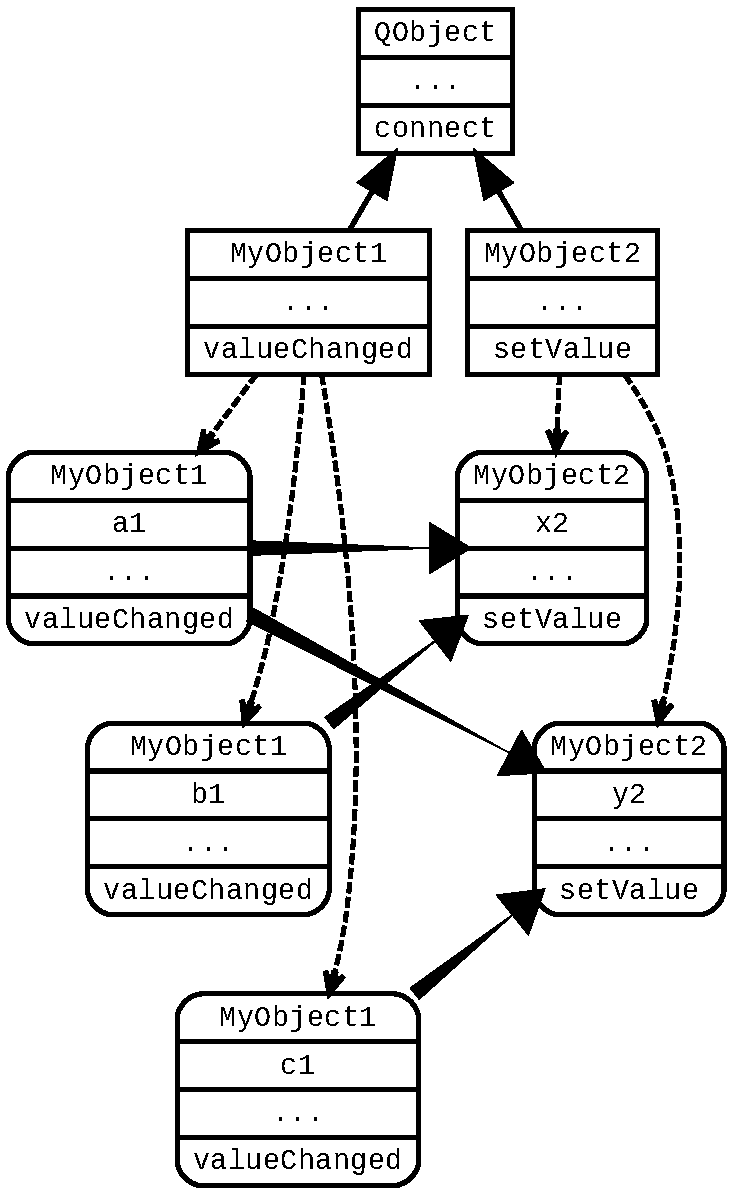
\includegraphics[width=\textwidth]{images/sig_slot_schema.pdf}
      \end{figure}
    \end{column}
  \end{columns}
\end{frame}

\begin{frame}[fragile]
  \frametitle{Disconnecting signals and slots}
   \small
   \begin{itemize}
      \item Purpose: disconnects \verb@this@ objects's named \verb@signal@
        connected to a named \verb@slot@ of a \verb@receiver@ object.
      \item Declaration (non-static)
      \begin{lstlisting}[basicstyle=\scriptsize\ttfamily]
	bool QObject::disconnect(
	    const char *signal = Q_NULLPTR,
	    const QObject *receiver = Q_NULLPTR,
	    const char *slot = Q_NULLPTR
	);
      \end{lstlisting}
      \item Usage
      \begin{lstlisting}[basicstyle=\scriptsize\ttfamily]
	QObject *sender = ..., *receiver = ...;
	sender->disconnect();
	sender->disconnect(SIGNAL(someSignal()));
	sender->disconnect(SIGNAL(someSignal()), receiver);
	sender->disconnect(Q_NULLPTR, receiver);
	sender->disconnect(
	    SIGNAL(someSignal()),
	    receiver, SLOT(someSlot())
	);
      \end{lstlisting}
    \end{itemize}
\end{frame}

\begin{frame}[fragile]
  \frametitle{Disconnecting signals and slots (cont.)}
   \small
   \begin{itemize}
      \item Purpose: disconnects the signals of \verb@this@ object
        connected to a named \verb@slot@ of a \verb@receiver@ object.
      \item Declaration (static)
      \begin{lstlisting}[basicstyle=\scriptsize\ttfamily]
	bool QObject::disconnect(
	    const QObject *receiver = Q_NULLPTR,
	    const char *slot = Q_NULLPTR
	);
      \end{lstlisting}
      \item Usage
      \begin{lstlisting}[basicstyle=\scriptsize\ttfamily]
	QObject *sender = ...;
	QObject *receiver = ...;
	QObject::disconnect(0, receiver, 0);
	QObject::disconnect(receiver, SLOT(someSlot()));
      \end{lstlisting}
    \end{itemize}
\end{frame}

\begin{frame}[fragile]
  \frametitle{Disconnecting signals and slots (cont.)}
   \small
   \begin{itemize}
      \item Purpose: disconnects named \verb@signal@ of \verb@sender@
        connected to a named \verb@slot@ of a \verb@receiver@ object.
      \item Declaration (static)
      \begin{lstlisting}[basicstyle=\scriptsize\ttfamily]
	bool QObject::disconnect(
	    const QObject *sender,
	    const char *signal = Q_NULLPTR,
	    const QObject *receiver = Q_NULLPTR,
	    const char *slot = Q_NULLPTR
	);
      \end{lstlisting}
      \item Usage
      \begin{lstlisting}[basicstyle=\scriptsize\ttfamily]
	QObject *sender = ..., *receiver = ...;
	QObject::disconnect(sender);
	QObject::disconnect(sender, SIGNAL(someSignal()));
	QObject::disconnect(sender, 0, receiver, 0);
	QObject::disconnect(
	    sender, SIGNAL(someSignal()),
	    receiver, SLOT(someSlot())
	);
      \end{lstlisting}
    \end{itemize}
\end{frame}

\begin{frame}[fragile]
  \frametitle{Disconnecting signals and slots (cont.)}
   \small
   \begin{itemize}
      \item Purpose: disconnects \verb@signal@ member function of \verb@sender@
        connected to a \verb@slot@ member function of a \verb@receiver@ object.
      \item Declaration (static)
      \begin{lstlisting}[basicstyle=\scriptsize\ttfamily]
	bool QObject::disconnect(
	    const QObject *sender,
	    PointerToMemberFunction signal,
	    const QObject *receiver,
	    PointerToMemberFunction slot
	);
      \end{lstlisting}
      \item Usage
      \begin{lstlisting}[basicstyle=\scriptsize\ttfamily]
	MyObject *sender = ..., *receiver = ...;
	QObject::disconnect(
	    sender, &MyObject::someSignal,
	    0, 0
	);
	QObject::disconnect(
	    sender, &MyObject::someSignal,
	    receiver, &MyObject::someSlot
	);
      \end{lstlisting}
    \end{itemize}
\end{frame}

\begin{frame}[fragile]
  \frametitle{Connection and disconnection notification}
   \small
   \begin{itemize}
      \item Connection notification
      \begin{itemize}
        \item \verb@QObject::connectNotify(const QMetaMethod& signal)@
        \begin{itemize}
          \item protected virtual member function
        \end{itemize}
        \item Called when a connection is made to \verb@this@ object's signal.
      \end{itemize}
      \item Disconnection notification
      \begin{itemize}
        \item \verb@QObject::disconnectNotify(const QMetaMethod&)@
        \begin{itemize}
          \item protected virtual member function
        \end{itemize}
        \item Called when a connection to \verb@this@ object's signal is disconnected.
      \end{itemize}
      \item Compare the \verb@signal@ argument to a specific signal:
      \begin{itemize}
        \item \verb@QMetaMethod::fromSignal()@
        \item
        \begin{lstlisting}[basicstyle=\tiny\ttfamily]
	if (signal == QMetaMethod::fromSignal(&MyObject::someSignal))
	{
	    /* ... */
	}
        \end{lstlisting}
      \end{itemize}
    \end{itemize}
\end{frame}

\begin{frame}[fragile]
  \frametitle{Events vs. Signals and slots}
  \small
  \begin{columns}
    \begin{column}{0.55\textwidth}
    \begin{itemize}
      \item Events:
      \scriptsize
      \begin{itemize}
      \item Lower-level mechanism.
      \item Messages encapsulated in objects.
      \item Events usually originate from external subsystems handling keyboard,
        mouse and sensor input and messages from the platform window system or OS.
      \item Handled by calling virtual member functions.
      \item Can be filtered and passed to other event handlers forming a chain.
      \item Usually only a single handler in the chain handles the event.
      \item Event handling requires sub-classing.
      \end{itemize}
    \end{itemize}
    \end{column}
    \begin{column}{0.45\textwidth}
    \begin{itemize}
      \item Signals and slots:
      \scriptsize
      \begin{itemize}
      \item Higher-level mechanism.
      \item \say{Special} member functions.
      \item Signals are \say{emitted} (called), connected slots are \say{notified}
        (called).
      \item When a signal is emitted, all slots are notified and respond to the
        signal independently.
      \item Signals are often emitted from Qt's default event handlers.
      \item Don't require sub-classing, but depend on the \verb@moc@-generated
        support code.
      \end{itemize}
    \end{itemize}
    \end{column}
  \end{columns}
\end{frame}

